\documentclass[main.tex]{subfiles}

\begin{document}

\subsection{Secondo esercizio}

\begin{figure}[htb]
\centering
\resizebox{.5\textwidth}{!}{ \providecommand{\main}{../../..}
\documentclass[\main/main.tex]{subfiles}
\begin{document}
\subsection{Esercizio 1}
Dato il seguente problema di PL, si risolva graficamente e si ottenga il valore della soluzione ottima e di tutte le variabili di scarto.

Vi sono vertici ammissibili ai quali corrispondono basi degeneri?

Si ricavi, per via grafica, per quali valori di $b_3$, inizialmente pari a $-1$, la \textbf{composizione} della base ottima non cambia.

\begin{figure}
  \begin{align*}
    \max \quad -x_1 + x_2 \\
    -x_1 -x_2   & \leq -2 \\
    -x_1 + 3x_2 & \leq 6  \\
    -2x_1 + x_2 & \leq -1 \\
    4x_1 - x_2  & \leq 20 \\
    2x_1 + x_2  & \leq 16 \\
    x_1, x_2    & \geq 0
  \end{align*}
  \caption{Esercizio 1}
\end{figure}

\subsection{Soluzione esercizio 1}
\subsubsection*{Disegno l'area di definizione del problema}
\begin{figure}
  \begin{subfigure}{0.45\textwidth}
    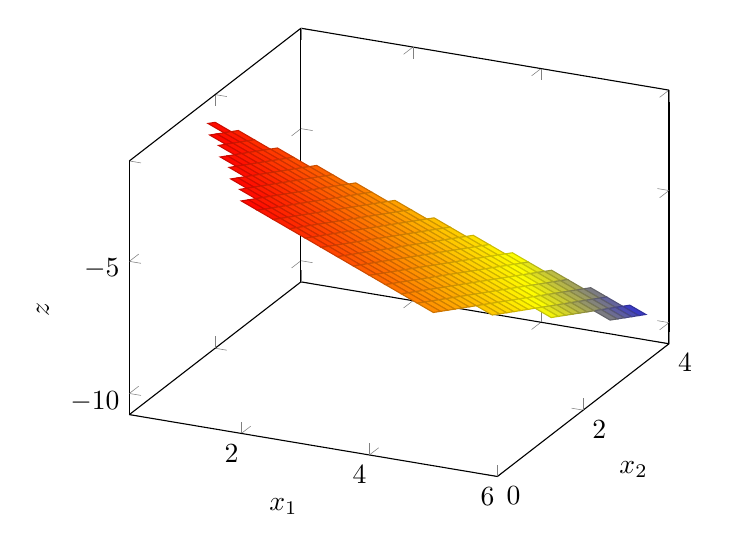
\begin{tikzpicture}
      \begin{axis}[
          xlabel=$x_1$,
          ylabel=$x_2$,
          zlabel=$z$,
          domain=0:6,
          y domain=0:4
        ]
        \addplot3[surf, unbounded coords=jump]
        {
          -x-y<=-2 &&
          -x +3*y <= 6 &&
          -2*x -y <= -1 &&
          4*x - y <= 20 &&
          2*x + y <= 16?
          -x-y:NaN
        };
      \end{axis}
    \end{tikzpicture}
    \caption{La funzione $z$}
  \end{subfigure}
  \begin{subfigure}{0.45\textwidth}
    \includegraphics[width=0.8\textwidth]{2017_01_1}
    \caption{Regione di definizione del problema}
  \end{subfigure}
\end{figure}

\subsubsection*{Identifico la soluzione ottima}
Dall'area di definizione e dalla composizione della funzione si intuisce che il vincolo ottimo sarà quello con $x_1$ minimo e $x_2$ massimo. Procedo quindi a calcolare il valore assunto da $x_1$ e $x_2$ nell'intersezione tra il vincolo $2$ e $3$:

\[
  \begin{cases}
    -x_1 + 3x_2  = 6 \\
    -2x_1 + x_2  = -1
  \end{cases}
  \Rightarrow
  \begin{cases}
    -x_1 + 3(2x_1 -1)  = 6 \\
    x_2  =2x_1 -1
  \end{cases}
  \Rightarrow
  \begin{cases}
    5x_1 -3  = 9 \Rightarrow x_1 = \frac{9}{5} \\
    x_2  =2x_1 -1 \Rightarrow x_2 = \frac{18-5}{5} = \frac{13}{5}
  \end{cases}
\]

La soluzione ottima si trova nel vertice tra il vincolo $2$ e $3$ in $(\frac{9}{5}, \frac{13}{5})$ ed ha valore $z = \frac{13}{5} - \frac{9}{5} = \frac{4}{5}$.

\subsubsection*{Identifico basi degeneri}
\begin{definition}[Determinante di matrice $2\times 2$]
  Risulta possibile calcolare il determinante di una matrice $A$ di dimensione $2 \times 2$ tramite la formula:
  \begin{figure}
    \[
      \det(A) = a_{11}a_{22} - a_{12}a_{21}
    \]
    \caption{Determinante di matrice $2 \times 2$}
  \end{figure}
\end{definition}

\begin{definition}[Inversa di matrice $2\times 2$]
  Risulta possibile ottenere l'inversa $A^{-1}$ di una matrice $A$ di dimensione $2 \times 2$ tramite la formula:
  \begin{figure}
    \[
      A^{-1} = \frac{1}{\det(A)} \begin{bmatrix}
        a_{22}  & -a_{21} \\
        -a_{12} & a_{11}  \\
      \end{bmatrix}
    \]
    \caption{Inversa di matrice $2 \times 2$}
  \end{figure}
\end{definition}

\begin{definition}[Base degenere]
  Una base $A_B$ è \textbf{degenere} quando nel risultato del vettore risultato del prodotto $A_B^{-1} \bm{b}$ appaiono degli 0.
\end{definition}

\begin{definition}[Base degenere $2 \times 2$] \label{degenere_2_2}
  Dato un vettore di risorse $\bm{b} = [b_1, b_2]$, una base $A_B$ di dimensione  $2 \times 2$ è \textbf{degenere} quando almeno una delle seguenti relazioni è vera:
  \[
    a_{11}b_2 - a_{12}b_1 = 0 \quad \lor \quad a_{22}b_1 - a_{21}b_2 = 0
  \]
\end{definition}

\paragraph*{Testo se il vertice tra il vincolo $1$ e $3$ è degenere:}

\begin{align*}
  v_1: -x_1 -x_2  & \leq -2 \\
  v_2: -2x_1 +x_2 & \leq -1
\end{align*}

La base così ottenuta è degenere se vale la relazione \ref{degenere_2_2}:

\[
  -1(-1) - (-1)(-2) \neq 0 \lor 1(-2) - (-2)(-1) = 0
\]
La seconda equazione è vera, pertanto questa base è degenere.

\subsubsection*{Analisi di sensitività}
Modifica il valore di $b_3$ significa traslare il vincolo $3$, che è uno dei due che definisce il punto di ottimo $(\frac{9}{5}, \frac{13}{5})$. Non è pertanto possibile alterare il valore di $b_3$ senza modificare il valore ottimo.

Per quanto riguarda la composizione della base ottima, essa rimane invariata tra $b_{3_{max}}$ dove il vincolo $v_3$ incontra il vincolo $v_1$ nel punto $(0,2)$ e $b_{3_{min}}$ dove il vincolo $v_3$ incrocia $v_4$ nel punto $(6,4)$. Per calcolare il valore assunto da $b_3$ nei due punti di interesse è sufficiente sostituire i punti nella disequazione del vincolo.

\[
  b_{3_{max}} = -2(0) + 1(2) = 2 \qquad b_{3_{min}} = -2(6) + 1(4) = -8
\]
\end{document}}
\caption{Isostatica con biella, incastro e cerniera con forza puntiforme}
\end{figure}

L'esercizio richiede di calcolare:
\begin{enumerate}
  \item Le reazioni vincolari a terra (in A) e nel punto C;
  \item Le azioni interne nell’asta AC.
\end{enumerate}

\subsection{Soluzione secondo esercizio}
\subsubsection{Osservazioni}
Prima di iniziare l'esercizio, è importante osservare che:
\begin{itemize}
  \item La struttura forma un triangolo equilatero.
  \item Possiede un unico punto A, che la vincola a terra.
  \item L'asta BD si comporta come una \textit{biella} o \textit{pendolo semplice}.
  \item Nella struttura son presenti $2$ corpi rigidi.
  \item Nella struttura son presenti 3 vincoli, una biella, una cerniera ed un incastro.
\end{itemize}
\subsubsection{Verifica preliminare di isostaticità}
Noi sappiamo risolvere solamente sistemi isostatici, per cui verifichiamo la condizione di isostaticità: $gdv_{totali} = gdl_{totali}$
\begin{gather*}
gdl_{totali}= 3 + 3 = 6
\end{gather*}
Ci aspettiamo quindi che i gradi di vincolo siano pari a $6$:
\begin{gather*}
gdv_{totali}= gdv_{biella} + gdv_{cerniera} + gdv_{incastro}
\end{gather*}
\subparagraph{Richiami sulle cerniere interne}
\begin{definition}[Cerniera interna]
Una cerniera è detta interna quando non è fissata a terra ed è compresa tra un numero $n$ di aste tale per cui:
\[ n>1 \]
\end{definition}
\begin{theorem}[Formula delle cerniere interne]
Una cerniera interna compresa tra $n$ aste impone un numero di gradi di vincolo pari a:
\[ gdv_{cerniera} = 2(n-1) \]
\end{theorem}

Per cui, sommando i gradi di vincolo di biella, cerniera ed incastro si ottiene:
\begin{gather*}
gdv_{totali}= 1 + 2(2-1) + 3 = 6
\end{gather*}

Quindi, in base all'analisi preliminare, la struttura è \textit{isostatica}.

\subparagraph{Limiti dell'analisi dei vincoli} L'analisi dei vincoli dà un risultato decisamente limitato: esistono infatti casi in cui la struttura risulta persino \textit{iperstatica} che in base ad un'analisi dei gradi di libertà risulterebbe \textit{labile}, cioè in grado di muoversi, e strutture che questa analisi descriverebbe \textit{iperstatiche} che in realtà son \textit{labili}.
Per vedere esempi di questi casi particolari, leggete la parte relativa alla statica nell'introduzione della dispensa.

In questo corso tuttavia, solo strutture \textit{isostatiche} son considerate, per cui non preoccupiamoci oltre.

\subsubsection{Primo punto}

\begin{figure}[htb]
\centering
\resizebox{.5\textwidth}{!}{ \providecommand{\main}{../../..}
\documentclass[\main/main.tex]{subfiles}
\begin{document}
\subsection{Esercizio 2}

\end{document}}
\caption{Analisi dei vincoli esterni}
\label{vincoli_esterni_1}
\end{figure}

\subparagraph{Vincoli esterni}
Iniziamo con l'analisi dei vincoli esterni (Figura \ref{vincoli_esterni_1}), che in questo caso sono unicamente A. Consideriamo quindi l'intero sistema come un corpo rigido, rimuovendo tutti i dettagli che non ci interessano e sostituiamo all'incastro in A le rispettive reazioni vincolari.

Normalmente, un vincolo ad incastro presenta 3 reazioni vincolari: una verticale ($V_A$), una orizzontale ($H_A$) ed un momento resistente ($M_A$) che si contrappone al momento imposto dalla forza esterna.

In questo caso, però, sul corpo rigido agisce una forza orientata sul piano orizzontale, senza alcuna componente verticale, per cui il vincolo a incastro non contrappone alcuna reazione verticale.

Inoltre il vettore $\vec{r}$, che rappresenta la distanza dal punto di applicazione della forza E al punto di applicazione del vincolo A, possiede unicamente una componente orizzontale, percui la forza esterna non va ad applicare alcun momento sul corpo rigido, essendo i due vettori paralleli.

Procedendo con le leggi di equilibrio della statica otteniamo:

\[
R_A : \begin{cases}
H_A - F = 0\\
V_A = 0\\
M_A = 0
\end{cases}
\Longrightarrow \begin{cases}
H_A = F\\
V_A = 0\\
M_A = 0
\end{cases}
\]

\begin{figure}[htb]
\centering
\resizebox{.5\textwidth}{!}{\providecommand{\main}{../../..}
\documentclass[\main/main.tex]{subfiles}
\begin{document}

\subsection{Exercise 3}
\begin{table}
  \begin{tabular}{L|LLLLL}
        & a_1 & a_2 & a_3 & a_4 & a_5 \\
    \hline
    f_1 & 0.5 & 1   & 0.6 & 0.3 & 0.2 \\
    f_2 & 0.4 & 0.1 & 0.2 & 0.3 & 0.7 \\
  \end{tabular}
\end{table}
\begin{enumerate}
  \item Explain the concept of paretian solution.
  \item Describe briefly the constrain method, making clear advantages and disadvantages.
  \item Describe briefly the weights method, making clear advantages and disadvantages.
  \item Determine the optimal solution from the given table with the utility function $u(f) = f_1f_2$.
\end{enumerate}

\end{document}}
\caption{Analisi dell'asta CE}
\label{vincoli_asta_CE_1}
\end{figure}

\subparagraph{Asta CE}
Ora per andare a calcolare le reazioni vincolari in C, andiamo a considerare l'asta CE e ne sostituiamo i vincoli con reazioni vincolari corrispondenti (figura \ref{vincoli_asta_CE_1}).

È importante ricordare che l'asta BD agisce da biella, e una biella trasmette unicamente la reazione assiale, indirizzata appunto con l'asse della biella.

Possiamo quindi notare che nulla agisce in direzione verticale sull'asta CE, per cui la C non impone una reazione verticale.

Procediamo nuovamente con la legge dell'equilibrio della statica, scegliendo (arbitrariamente\footnote{generalmente si sceglie il punto con più forze applicate, così che non debbano essere considerate per semplificare l'equazione dell'equilibrio dei momenti. In questo caso in tutti i punti vi è applicata al più una forza, per cui è indifferente. Oltre a questo motivo, se fosse presente un momento (applicato dall'esterno, o presente per via di un momento resistente) verrebbe scelto il punto in cui vi è il momento.}) come punto in cui calcolare l'equilibrio dei momenti il punto C, otteniamo:

\[
R_C : \begin{cases}
H_C + R_D - F = 0\\
V_C = 0\\
M_C = 0 = LR_D - 2LF
\end{cases}
\Longrightarrow \begin{cases}
H_C = F - R_D\\
V_C = 0\\
R_D = 2F
\end{cases}
\Longrightarrow \begin{cases}
H_C = -F\\
V_C = 0\\
R_D = 2F
\end{cases}
\]

Siccome $\vec{H_C}$ è risultato negativo, ne abbiamo scelto una direzione "sbagliata". Poco male. Correggiamo quindi la figura, per avere un'immagine che meglio rifletta la realtà (figura \ref{vincoli_asta_CE_2}):


\begin{figure}[!tbp]
  \begin{subfigure}[b]{.5\textwidth}
  \centering
  \resizebox{.5\textwidth}{!}{ \providecommand{\main}{../../..}
\documentclass[\main/main.tex]{subfiles}
\usetikzlibrary{graphdrawing}
\usetikzlibrary{graphs}
\usegdlibrary{trees}
\begin{document}
\subsection{Esercizio 4}
Si risolva mediante Branch \& Bound il seguente problema dello zaino a capacità massima 9, seguendo le istruzioni seguenti:

\begin{table}
  \begin{tabular}{c|LLLLL}
    Profitti & 21 & 10 & 20 & 4 & 3 \\
    \hline
    Pesi     & 3  & 2  & 5  & 2 & 3
  \end{tabular}
\end{table}

\begin{enumerate}
  \item Si utilizzi come rilassamento quello lineare, risolto mediante un opportuno algoritmo.
  \item Si adotti una strategia ``Depth First''.
  \item Si esplori per primo ad ogni livello il ramo dell'albero di branching associato al vincolo $x_i=0$, dove la variabile di branching $x_i$ è quella che assume un valore frazionario nel rilassamento lineare.
  \item È possibile fissare a zero una variabile qualora la capacità residua dello zaino sia strettamente minore del suo peso.
  \item Come \textbf{lower bound} si usi la miglior soluzione intera data dalla somma dei profitti degli oggetti che è stato possibile inserire nello zaino durante il calcolo dell'\textbf{upper bound}.
  \item Per ogni nodo si riportino:
        \subitem Numero progressivo $i$.
        \subitem Valore di upper bound.
        \subitem Valore del vettore delle variabili.
\end{enumerate}

\subsection{Soluzione esercizio 4}
\begin{figure}
  \begin{tikzpicture}
    \Tree[.\text{$0:\begin{cases}
            \bmx=\sqr{0,0,0,0,0} \\
            U=47
          \end{cases}$}
      [.$x_1=0$
        [.\text{$1:\begin{cases}
                  1:\bmx=\sqr{0,0,0,0,0} \\
                  U=34
                \end{cases}$}
            [.$x_2=0$
              [.\text{$2:\begin{cases}
                        \bmx=\sqr{0,0,0,0,0} \\
                        U=26
                      \end{cases}$}
                  [.$x_3=0$
                    [.\text{$3:\begin{cases}
                              \bmx=\sqr{0,0,0,1,1} \\
                              z=7
                            \end{cases}$} ]
                  ]
                  [.$x_3=1$
                    [.\text{$4:\begin{cases}
                              \bmx=\sqr{0,0,1,0,0} \\
                              U=26
                            \end{cases}$}
                        [.$x_4=0$
                          [.\text{$5:\begin{cases}
                                    \bmx=\sqr{0,0,1,0,1} \\
                                    z=23
                                  \end{cases}$} ]
                        ]
                        [.$x_4=1$
                          [.\text{$6:\begin{cases}
                                    \bmx=\sqr{0,0,1,1,0} \\
                                    z=24
                                  \end{cases}$} ]
                        ]
                      ]
                  ]
                ]
            ]
            [.$x_2=1$
              [.\text{$4:\begin{cases}
                        \bmx=\sqr{0,1,1,0,0} \\
                        U=26
                      \end{cases}$}
                  [.$x_4=0$
                    [.\text{$5:\begin{cases}
                              \bmx=\sqr{0,1,1,0,1} \\
                              z=23
                            \end{cases}$} ]
                  ]
                  [.$x_4=1$
                    [.\text{$6:\begin{cases}
                              \bmx=\sqr{0,0,1,1,0} \\
                              z=24
                            \end{cases}$} ]
                  ]
                ]
            ]
          ]
      ]
    ]
  \end{tikzpicture}
\end{figure}
\end{document}}
  \caption{Asta CE con reazioni vincolari.}
  \end{subfigure}
  \hfill
  \begin{subfigure}[b]{.5\textwidth}
  \centering
  \resizebox{.5\textwidth}{!}{\providecommand{\main}{../../..}
\documentclass[\main/main.tex]{subfiles}
\begin{document}

\subsection{Exercise 6}
Model and resolve the following decision problem in uncertainty conditions.

We want to order a pizza from a distant restaurant that sells it at \$10. It is possible to get it personally or to request the home delivery, which costs \$2, with a probability of the 2\% that the delivery delays and the pizza gets cold. In this scenario the pizza is free, and we can either choose to eat it as such with a discomfort measurable as a expenditure of \$5 or to heat it up again in the home oven, with a probability of the 10\% to burn it and having to go to the restaurant downstairs, where a pizza costs \$15.

If one choses to retrieve the pizza by himself, there's a probability of the 10\% that the pizza gets cold. In this scenario, one can either eat it cold with a discomfort of \$5 or ask to the restaurant for having it re-heated, with a cost of \$1 and a discomfort measurable as an expenditure of \$1.

\subsection{Exercise 6 resolution}
\begin{figure}
  \begin{tikzpicture}
    \Tree[.root
    [.\text{Home delivery}
    [.\text{2\%: The pizza gets cold}
    [.\text{Eat it cold}
    [.\$5 ]
    ]
    [.\text{Try to re-heat it}
    [.{10\%: The pizza gets burned}
    [.\text{You have to buy it downstairs}
    [.\$15 ]
    ]
    ]
    [.{90\%: The pizza is heated}
    [.\$0 ]
    ]
    ]
    ]
    [.\text{98\%: The pizza is fine}
    [.\$10 ]
    ]
    ]
    [.\text{Personal retrieval}
    [.\text{10\% You are late}
      [.\text{Eat it cold}
        [.\$15 ]
      ]
      [.\text{Re-heat it}
        [.\$12 ]
      ]
    ]
    [.\text{90\% You are on time}
      [.\$10 ]
    ]
    ]
    ]
  \end{tikzpicture}
\end{figure}

Resolving the tree with optimizing for minimum cost.

\begin{figure}
  \begin{tikzpicture}
    \Tree[.root
    [.\text{Home delivery}
    [.\text{2\%: The pizza gets cold}
    [.\text{Eat it cold}
    [.\$5 ]
    ]
    [.\text{Try to re-heat it}
    [.{10\%: The pizza gets burned}
    [.\text{You have to buy it downstairs}
    [.\$15 ]
    ]
    ]
    [.{90\%: The pizza is heated}
    [.\$0 ]
    ]
    ]
    ]
    [.\text{98\%: The pizza is fine}
    [.\$10 ]
    ]
    ]
    [.\text{Personal retrieval}
    [.\text{10\% You are late}
      [.\text{Re-heat it}
        [.\$12 ]
      ]
    ]
    [.\text{90\% You are on time}
      [.\$10 ]
    ]
    ]
    ]
  \end{tikzpicture}
\end{figure}

\begin{figure}
  \begin{tikzpicture}
    \Tree[.root
    [.\text{Home delivery}
    [.\text{2\%: The pizza gets cold}
      [.\text{Eat it cold}
        [.\$5 ]
      ]
      [.\text{Try to re-heat it}
        [.\$1.5 ]
      ]
    ]
    [.\text{98\%: The pizza is fine}
      [.\$10 ]
    ]
    ]
    [.\text{Personal retrieval}
    [.\$10.2 ]
    ]
    ]
  \end{tikzpicture}
\end{figure}

\begin{figure}
  \begin{tikzpicture}
    \Tree[.root
    [.\text{Home delivery}
    [.\text{2\%: The pizza gets cold}
      [.\text{Try to re-heat it}
        [.\$1.5 ]
      ]
    ]
    [.\text{98\%: The pizza is fine}
      [.\$10 ]
    ]
    ]
    [.\text{Personal retrieval}
    [.\$10.2 ]
    ]
    ]
  \end{tikzpicture}
\end{figure}

\begin{figure}
  \begin{tikzpicture}
    \Tree[.root
    [.\text{Home delivery}
    [.\$9.83 ]
    ]
    [.\text{Personal retrieval}
    [.\$10.2 ]
    ]
    ]
  \end{tikzpicture}
\end{figure}


\begin{figure}
  \begin{tikzpicture}
    \Tree[.root
    [.\text{Home delivery}
    [.\$9.83 ]
    ]
    ]
  \end{tikzpicture}
\end{figure}

\end{document}
}
  \caption{Asta CE con modulo della forza esterna.}
  \end{subfigure}
  \caption{Analisi corretta dell'asta CE.}
  \label{vincoli_asta_CE_2}
\end{figure}
\subparagraph{Ricapitolo primo punto}

\[
R_A : \begin{cases}
H_A = F\\
V_A = 0\\
M_A = 0
\end{cases}
;
R_C : \begin{cases}
H_C = F\\
V_C = 0\\
M_C = 0
\end{cases}
\]

\begin{figure}[!tbp]
  \begin{subfigure}[b]{.5\textwidth}
  \centering
  \resizebox{.5\textwidth}{!}{\providecommand{\main}{../../..}
\documentclass[\main/main.tex]{subfiles}
\begin{document}

\subsection{Esercizio 5}
Viene dato il seguente problema di programmazione in condizioni di incertezza, i cui valori indicano utilità:

\begin{table}
  \begin{tabular}{|L|L|L|L|L|}
    \hline
    u_{\omega a} & a_1 & a_2 & a_3 & a_4 \\
    \hline
    \omega_1     & 50  & 40  & 60  & 90  \\
    \hline
    \omega_1     & 10  & 30  & 20  & 0   \\
    \hline
  \end{tabular}
\end{table}

\begin{enumerate}[a)]
  \item Si indichi se vi sono alternative dominate e quali alternative le dominano.
  \item Si indichi l’alternativa scelta con il criterio del caso pessimo.
  \item Si mostri come cambia l’alternativa scelta con il criterio del caso medio al variare della probabilità $\pi(\omega_1)$ del primo scenario.
\end{enumerate}

\subsection{Soluzione esercizio 5}
\subsubsection*{Alternative dominate}
Un'alternativa domina un'altra quando, senza applicare particolari criteri, questa è migliore per almeno uno degli scenari ed uguale in tutti gli altri.

Cerchiamo la soluzione che dia scenari a valore massimo poichè i valori rappresentano utilità.

In questo caso, l'alternativa solamente $a_3 \prec a_1$, mentre non è possibile affermare nulla delle altre che sono preferibili l'una alle altre per almeno uno scenario.

\subsubsection*{Criterio del caso pessimo}
Nel criterio del caso pessimo, si assume che qualsiasi scelta venga effettuata accadrà il suo corrispondente caso pessimo.

\begin{table}
  \begin{tabular}{|L|L|L|L|L|}
    \hline
    u_{\omega a} & a_1                   & a_2                   & a_3                   & a_4                 \\
    \hline
    \omega_1     & 50                    & 40                    & 60                    & 90                  \\
    \hline
    \omega_1     & \cellcolor{red!50} 10 & \cellcolor{red!50} 30 & \cellcolor{red!50} 20 & \cellcolor{red!50}0 \\
    \hline
  \end{tabular}
  \caption{Casi pessimi in rosso}
\end{table}

La scelta con scenario pessimo migliore è $a_2$.

\subsubsection*{Caso medio}
Il caso medio (suppongo sia, dato che non appare nelle dispense) il caso di equiprobabilità con coefficiente pari $\pi(\omega_1)$ per il primo scenario e $1-\pi(\omega_1)$ per il secondo.

\begin{table}
  \begin{tabular}{|L|L|L|L|L|}
    \hline
        & a_1                                   & a_2                                   & a_3                                   & a_4             \\
    \hline
    u_L & 50\pi(\omega_1) + 10(1-\pi(\omega_1)) & 40\pi(\omega_1) + 30(1-\pi(\omega_1)) & 60\pi(\omega_1) + 20(1-\pi(\omega_1)) & 90\pi(\omega_1) \\
    \hline
  \end{tabular}
\end{table}

\begin{figure}
  \begin{subfigure}{0.31\textwidth}
    \begin{table}[H]
      \begin{tabular}{|L|L|L|L|L|}
        \hline
            & a_1 & a_2 & a_3 & a_4 \\
        \hline
        u_L & 50  & 40  & 60  & 90  \\
        \hline
      \end{tabular}
      \caption{Caso $\pi(\omega_1)=1$: viene scelta $a_4$}
    \end{table}
  \end{subfigure}
  \begin{subfigure}{0.31\textwidth}
    \begin{table}[H]
      \begin{tabular}{|L|L|L|L|L|}
        \hline
            & a_1 & a_2 & a_3 & a_4 \\
        \hline
        u_L & 10  & 30  & 20  & 0   \\
        \hline
      \end{tabular}
      \caption{Caso $\pi(\omega_1)=0$: scelta $a_2$}
    \end{table}
  \end{subfigure}
  \begin{subfigure}{0.31\textwidth}
    \begin{tikzpicture}
      \begin{axis}[
          width= \textwidth,
          xlabel=$f$,
          ylabel=$u_L$,
          domain=0:1,
          ytick = {0,10,...,90},
          legend style={at={(0,1)},anchor=north west}
        ]
        \addplot[mark=none,color=red]{50*x + 10*(1-x)};
        \addplot[mark=none,color=blue]{40*x + 30*(1-x)};
        \addplot[mark=none,color=green]{60*x + 20*(1-x)};
        \addplot[mark=none]{90*x};
        \legend{$a_1$,$a_2$,$a_3$,$a_4$}
      \end{axis}
    \end{tikzpicture}
    \caption{L'utilità $u_L$ al variare della probabilità}
  \end{subfigure}
\end{figure}



\end{document}
}
  \caption{Reazioni vincolari nell'asta AC.}
  \end{subfigure}
  \hfill
  \begin{subfigure}[b]{.5\textwidth}
  \centering
  \resizebox{.5\textwidth}{!}{\providecommand{\main}{../../..}
\documentclass[\main/main.tex]{subfiles}
\begin{document}

\subsection{Esercizio 7}
Si determini la soluzione ottima con la funzione di utilità $u = \w_1f_1 + \w_2f_2$ con $\w_1 = 0.25$ e $\w_2 = 0.75$ del seguente problema di programmazione a due obbiettivi:

\begin{figure}
  \begin{align*}
    \max f_1 = -x_1 + 2x_2 \\
    \max f_1 = 2x_1 - x_2  \\
    x_1 + x_2  & \leq 7    \\
    -x_1 + x_2 & \leq 3    \\
    x_1 - x_2  & \leq 3    \\
    x_1, x_2   & \leq 4    \\
    x_1, x_2   & \geq 0
  \end{align*}
  \caption{Esercizio 7}
\end{figure}

Si supponga ora di aggiungere un terzo obbiettivo, anch'esso da massimizzare $f_3 = 2x_1 + x_2$ e si disegnino nel piano $\w_1-\w_2$ le regioni nelle quali ciascuna soluzione di base ammissibile del problema lineare risulta ottima.

\subsection{Soluzione esercizio 7}

\subsubsection*{Costruisco funzione obbiettivo}

\[
  u = 0.25(-x_1 + 2x_2) + 0.75(2x_1-x_2) = 1.25x_1 + 0.75x_2
\]
\subsubsection*{Risolvo il problema lineare con la nuova funzione obbiettivo}

\begin{align*}
  u^* = 1.25x_1 - 0.25x_2 \\
  x_1 + x_2  & \leq 7     \\
  -x_1 + x_2 & \leq 3     \\
  x_1 - x_2  & \leq 3     \\
  x_1, x_2   & \leq 4     \\
  x_1, x_2   & \geq 0
\end{align*}
La variabile con cofficiente massimo è $x_1$, che può assumere al massimo valore $4$. Il valore di $x_2$ è invece da minimizzare, e può assumere valore minimo $1$ se fissiamo $x_1=4$.

\subsubsection*{Verifico la soluzione}

\begin{figure}
  \begin{subfigure}{0.45\textwidth}
    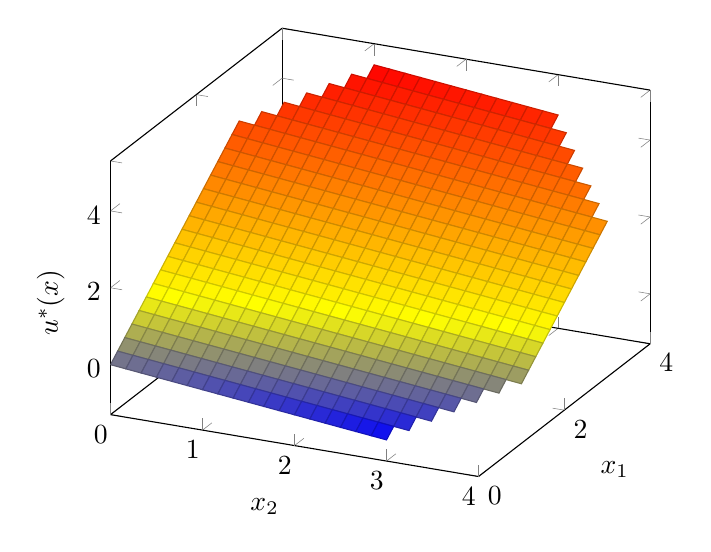
\begin{tikzpicture}
      \begin{axis}[
          xlabel=$x_2$,
          ylabel=$x_1$,
          zlabel=$u^*(x)$,
          domain=0:4,
          y domain=0:4
        ]
        \addplot3[surf, unbounded coords=jump]
        {x+y<=7 && x-y <= 3 && -x+y <= 3 ? 1.25*y - 0.25*x : NaN};
      \end{axis}
    \end{tikzpicture}
    \caption{La funzione $u^*(x)$}
  \end{subfigure}
  ~
  \begin{subfigure}{0.45\textwidth}
    \includegraphics[width=0.8\textwidth]{es7-maut}
    \caption{Dominio della funzione $u^*(x)$}
  \end{subfigure}
\end{figure}

\subsubsection*{Aggiungo funzione obbiettivo aggiuntiva}
Considerando il peso di $w_3 = 1- \w_1 - \w_2$ e $\w_1+\w_2\leq1$, procedo ad identificare le soluzioni ottime al variare dei pesi.

La nuova funzione obbiettivo risulta:

\[
  u' = \w_1(-x_1 + 2x_2) + \w_2(2x_1 - x_2) + (1 - \w_1 -\w_2)(2x_1 + x_2) = \w_1(-3x_1 + x_2) - 2\w_2x_2 + 2x_1 + x_2
\]

\begin{figure}
  \includegraphics[width=0.4\textwidth]{es7-maut}
  \caption{Area di definizione}
\end{figure}

I vertici sono in $v_1 = (0,3), v_2 = (1,4), v_3 = (3,4), v_4=(4,3), v_5=(4,1), v_6=(3,0)$ e $v_7 = (0,0)$.

Il vertice $v_7$ non può mai essere soluzione ottima, essendo tutte le funzioni di massimo.

Per risolvere l'esercizio è sufficiente risolvere i seguenti sistemi 6 lineari.

\begin{align*}
  -6y + 3     & \geq\max\rnd{-6y + 3,-x-4y + 4,-5x-8y + 10,-9x-6y + 11,-11x-2y + 9,-9x+ 6} \\
  -x-4y + 4   & \geq\max\rnd{-6y + 3,-x-4y + 4,-5x-8y + 10,-9x-6y + 11,-11x-2y + 9,-9x+ 6} \\
  -5x-8y + 10 & \geq\max\rnd{-6y + 3,-x-4y + 4,-5x-8y + 10,-9x-6y + 11,-11x-2y + 9,-9x+ 6} \\
  -9x-6y + 11 & \geq\max\rnd{-6y + 3,-x-4y + 4,-5x-8y + 10,-9x-6y + 11,-11x-2y + 9,-9x+ 6} \\
  -11x-2y + 9 & \geq\max\rnd{-6y + 3,-x-4y + 4,-5x-8y + 10,-9x-6y + 11,-11x-2y + 9,-9x+ 6} \\
  -9x+ 6      & \geq\max\rnd{-6y + 3,-x-4y + 4,-5x-8y + 10,-9x-6y + 11,-11x-2y + 9,-9x+ 6} \\
\end{align*}

Mi limito a plottare il risultato calcolato dal computer.

\begin{figure}
  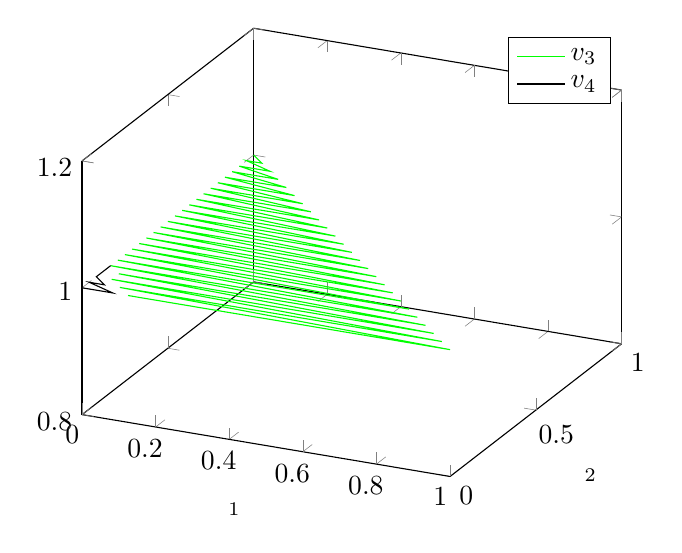
\begin{tikzpicture}
    \begin{axis}[
        xlabel=$\w_1$,
        ylabel=$\w_2$,
        domain=0:1,
        y domain=0:1
      ]

      % \addplot3[mark=none,color=pink]{-6*y + 3\geq=max(-6*y + 3,-x-4*y + 4,-5*x*-8*y + 10,-9*x-6*y + 11,-11*x-2*y + 9,-9*x+ 6)-0.1?1:NaN};
      % \addplot3[mark=none,color=blue]{-x-4*y + 4>=max(-6*y + 3,-x-4*y + 4,-5*x*-8*y + 10,-9*x-6*y + 11,-11*x-2*y + 9,-9*x+ 6)-0.1?1:NaN};
      \addplot3[mark=none,color=green]{x+y<=1 && -5*x*-8*y + 10>=max(-6*y + 3,-x-4*y + 4,-5*x*-8*y + 10,-9*x-6*y + 11,-11*x-2*y + 9,-9*x+ 6)?1:NaN};
      \addplot3[mark=none,color=black]{x+y<=1 && -9*x-6*y + 11>=max(-6*y + 3,-x-4*y + 4,-5*x*-8*y + 10,-9*x-6*y + 11,-11*x-2*y + 9,-9*x+ 6)?1:NaN};
      \addplot3[mark=none,color=red]{x+y<=1 && -11*x-2*y + 9>=max(-6*y + 3,-x-4*y + 4,-5*x*-8*y + 10,-9*x-6*y + 11,-11*x-2*y + 9,-9*x+ 6)?1:NaN};
      \addplot3[mark=none,color=blue]{x+y<=1 && -9*x+ 6>=max(-6*y + 3,-x-4*y + 4,-5*x*-8*y + 10,-9*x-6*y + 11,-11*x-2*y + 9,-9*x+ 6)?1:NaN};

      % \legend{$v_1$,$v_2$,$v_3$,$v_4$,$v_5$,$v_6$}
      \legend{$v_3$,$v_4$,$v_5$,$v_6$}
    \end{axis}
  \end{tikzpicture}

\end{figure}
\end{document}}
  \caption{Asta AC con modulo della forza esterna.}
  \end{subfigure}
  \caption{Analisi dell'asta AC.}
  \label{vincoli_asta_AC_1}
\end{figure}

\subsubsection{Secondo punto}
Per calcolare le azioni interne dell'asta AC, iniziamo disegnando le reazioni vincolari (e le forze e momenti applicati, se vi fossero) che la caratterizzano (figura \ref{vincoli_asta_AC_1}). Riassumendo, sull'asta AC agiscono:

In B agisce la reazione assiale $\vec{R_D} = \vec{R_B}$ (pari ed opposta a quanto vista nell'asta CE in D);

In C agisce la reazione vincolare $\vec{H_C}$;

In A agisce la reazione vincolare $\vec{H_A}$;

\subfile{nota_componenti_vettore.tex}

\paragraph{Divisione in componenti}
Separiamo ora le singole componenti in taglio e sforzo normale.

\begin{figure}[htb]
\centering
\resizebox{.5\textwidth}{!}{\providecommand{\main}{../../..}
\documentclass[\main/main.tex]{subfiles}
\begin{document}

\subsection{Exercise 8}
\begin{enumerate}[a)]
	\item Describe the concept of constitution as a method to aggregate preferences.
	\item Describe the plurality system method to aggregate preferences.
	\item Describe the concept of decisive set for a tuple of impacts $(f, f')$.
	\item Describe the concept of dependency from irrelevant alternatives, explaining why one would try to avoid it in group decision.
\end{enumerate}

\subsection{Exercise 8 resolution}
\subsubsection*{Constitution}
A constitution is a function that associates to every set of weak orders relationships on a given set of solutions or alternatives a weak order relationship of the group on the same set of solutions.

\subsubsection*{Plurality system}
The alternative that is more commonly accepted as the optimal by the decision makers. In case of a draw, the solution less commonly accepted is eliminated and the process is repeated.

This method has the defect that it allows solutions strongly desired by a minority and just slightly wanted by a majority to win.

\subsubsection*{Decisive set}
The group of decision makers that makes a given impact preferable to a second one in the group weak order.

\subsubsection*{Dependency from weak alternatives}
The concept of dependency from weak alternatives describe the situation when a value function bonds the value of a better alternative to the existence of a worst one, for example the method of Borda. This can lead to the \textbf{rank reversal}, a phenomenon for which the optimal solution can vary when one deletes the worst one.

It is one of the most common issues in politics, when the order a set of laws is approved or not changes which laws are approved.

\end{document}}
\caption{Componenti nell'asta AC}
\label{separated_components_1}
\end{figure}

\subparagraph{Calcolo dello sforzo normale}
Procediamo al calcolo della componente di sforzo normale di ogni forza applicata all'asta AC:
\[
	N: \begin{cases}
		\vec{N_A} = H_A\cos(\frac{\pi}{3})\\
		\vec{N_B} = R_B\cos(-\frac{\pi}{3})\\
		\vec{N_C} = H_C\cos(\frac{\pi}{3})
	\end{cases}
	\Longrightarrow
	\begin{cases}
		\vec{N_A} = \frac{1}{2}F\\
		\vec{N_B} = F\\
		\vec{N_C} = \frac{1}{2}F
	\end{cases}
\]

\subparagraph{disegniamo il grafico dello sforzo normale}
Ricordando la convenzione dello sforzo normale, \textbf{positivo} quando produce \textit{trazione} e \textbf{negativo} quando produce \textit{contrazione},  procediamo al disegno del grafico:

Mentre si disegna un grafico di questo tipo, è importante ricordare che il grafico deve risultare, quando è verticale, di un'altezza pari al vettore che agisce in quel punto. Per esempio, nel punto B il grafico ha un'altezza complessiva pari al valore di $N_B$, così come è analogamente in A ed in C.

Si può iniziare a disegnare il grafico partendo da un qualsiasi estremo del corpo rigido.

Iniziamo per esempio dall'estremo A. Spostiamoci di un $ds$ verso l'alto e osserviamo per questo \textit{concio elementare} se lo sforzo normale sia di trazione o contrazione. In questo caso, lo sforzo è di contrazione, per cui nella nostra convenzione definiamo il valore come negativo. Procedendo via via lungo l'asta, arriviamo al punto B, in cui è applicata una nuova forza. Qui, sommiamo i due valori dello sforzo e procediamo oltre. Da questo punto, siccome $N_B>N_A$ lo sforzo diviene di trazione e così rimane sino alla fine dell'asta in C.

Come già detto, se si esegue la stessa operazione partendo dall'estremo C al posto che in A si \textit{deve} ottenere lo stesso risultato.

\begin{figure}[!tbp]
  \begin{subfigure}[b]{.5\textwidth}
  \centering
  \resizebox{.5\textwidth}{!}{\input{chapters/2/2015/0629/2/sforzi_baricentrici.tex}}
  \caption{Sforzi normali baricentrici in AC.}
  \end{subfigure}
  \hfill
  \begin{subfigure}[b]{.5\textwidth}
  \centering
  \resizebox{.5\textwidth}{!}{\input{chapters/2/2015/0629/2/grafico_sforzi_baricentrici.tex}}
  \caption{Grafico dello sforzo normale.}
  \end{subfigure}
  \caption{Analisi dello sforzo normale nell'asta AC.}
\end{figure}

\subparagraph{Calcolo del taglio}
Procediamo al calcolo della componente di taglio di ogni forza applicata all'asta AC:

\[
	T: \begin{cases}
		\vec{T_A} = H_A\sin(\frac{\pi}{3})\\
		\vec{T_B} = R_B\sin(-\frac{\pi}{3})\\
		\vec{T_C} = H_C\sin(\frac{\pi}{3})
	\end{cases}
	\Longrightarrow
	\begin{cases}
		\vec{T_A} = \frac{\sqrt{3}}{2}F\\
		\vec{T_B} = -\sqrt{3}F\\
		\vec{T_C} = \frac{\sqrt{3}}{2}F
	\end{cases}
\]

\subparagraph{disegniamo il grafico del taglio}
Ricordando la convenzione del taglio, \textbf{positivo} quando produce \textit{rotazione oraria} e \textbf{negativo} quando produce \textit{rotazione anti-oraria},  procediamo al disegno del grafico:

Mentre si disegna un grafico di questo tipo, è importante ricordare che il grafico deve risultare, quando è verticale, di un'altezza pari al vettore che agisce in quel punto. Per esempio, nel punto B il grafico ha un'altezza complessiva pari al valore di $T_B$, così come è analogamente in A ed in C.

Si può iniziare a disegnare il grafico partendo da un qualsiasi estremo del corpo rigido.

Iniziamo per esempio dall'estremo A. Spostiamoci di un $ds$ verso l'alto e osserviamo per questo \textit{concio elementare} se il taglio produca rotazione oraria o anti-oraria. In questo caso, produce una rotazione anti-oraria. Procedendo via via lungo l'asta, arriviamo al punto B, in cui è applicata una nuova forza. Qui, sommiamo i due valori del taglio e procediamo oltre. Da questo punto, siccome $T_B>T_A$ il taglio produce una rotazione oraria e così rimane sino alla fine dell'asta in C.

Come già detto, se si esegue la stessa operazione partendo dall'estremo C al posto che in A si \textit{deve} ottenere lo stesso risultato.

\begin{figure}[!tbp]
  \begin{subfigure}[b]{.5\textwidth}
  \centering
  \resizebox{.5\textwidth}{!}{\input{chapters/2/2015/0629/2/taglio_AC.tex}}
  \caption{Taglio in AC.}
  \end{subfigure}
  \hfill
  \begin{subfigure}[b]{.5\textwidth}
  \centering
  \resizebox{.5\textwidth}{!}{\input{chapters/2/2015/0629/2/grafico_taglio_AC.tex}}
  \caption{Grafico del taglio.}
  \end{subfigure}
  \caption{Analisi del taglio nell'asta AC.}
\end{figure}

\subparagraph{Calcolo del momento flettente}
Procediamo al calcolo della componente del momento flettente. Scegliamo, per esempio, A come punto di origine del nostro calcolo del momento flettente. Un qualsiasi altro estremo dovrà dare lo stesso risultato.

La forza normale all'asta (che in questo caso è $T_A$) che viene applicata in A, se per un attimo immaginiamo l'asta come duttile, \textit{piega l'asta verso destra}. In A quindi, le fibre saranno \textit{tese sul lato di sinistra}.

Chiamiamo $\Delta{S}$ la distanza dal punto A. Il momento, in un generico punto tra A e B, sarà pari quindi a $M = \Delta{S}T_A$. Quando arriviamo in B, viene introdotta un'altra forza normale all'asta, $T_B$, di direzione opposta. Chiamiamo la distanza dal punto B $\Delta{k}$ e procediamo. Questo porta il momento a divenire pari a $M = \Delta{S}T_A - \Delta{K}T_B$, e gradualmente riduce il valore del momento sino ad azzerarsi in C.

Come già detto, se si esegue la stessa operazione partendo dall'estremo C al posto che in A si \textit{deve} ottenere lo stesso risultato.

\[
	M_{max} = \Delta{S}_{M_{max}}T_A = LT_A = L\frac{\sqrt{3}}{2}F
\]

\begin{figure}[!tbp]
  \begin{subfigure}[b]{.5\textwidth}
  \centering
  \resizebox{.5\textwidth}{!}{\input{chapters/2/2015/0629/2/taglio_AC.tex}}
  \caption{Forze che producono momento flettente in AC.}
  \end{subfigure}
  \hfill
  \begin{subfigure}[b]{.5\textwidth}
  \centering
  \resizebox{.5\textwidth}{!}{\input{chapters/2/2015/0629/2/grafico_momento_AC.tex}}
  \caption{Grafico del momento flettente.}
  \end{subfigure}
  \caption{Analisi del momento flettente nell'asta AC.}
\end{figure}

\paragraph{Visualizzazione della sovrapposizione degli effetti}
Questo può essere un utile strumento per visualizzare l'effetto di ogni singola forza, anche se in alcune combinazioni questi effetti considerati uno per volta possono non avere una reale controparte fisica.

\subparagraph{Sovrapposizione degli effetti per lo sforzo normale}
Disegnando l'effetto di una sola forza per volta (figura \ref{sforzo_forza_singola}), l'effetto delle forze accoppiate due a due  (figura \ref{sforzo_coppia_forze}) si capisce come l'applicazione di forze diverse in punti diversi vada a imporre uno sforzo normale differente.

\begin{figure}[!tbp]
  \begin{subfigure}[b]{.3\textwidth}
  \centering
  \resizebox{.5\textwidth}{!}{\input{chapters/2/2015/0629/2/grafico_sforzo_A.tex}}
  \caption{Sforzo normale di $N_A$.}
  \end{subfigure}
  \hfill
  \begin{subfigure}[b]{.3\textwidth}
  \centering
  \resizebox{.5\textwidth}{!}{\input{chapters/2/2015/0629/2/grafico_sforzo_B.tex}}
  \caption{Sforzo normale di $N_B$.}
  \end{subfigure}
  \hfill
  \begin{subfigure}[b]{.3\textwidth}
  \centering
  \resizebox{.5\textwidth}{!}{\input{chapters/2/2015/0629/2/grafico_sforzo_C.tex}}
  \caption{Sforzo normale di $N_C$.}
  \end{subfigure}
  \caption{Sforzo normale delle singole forze.}
  \label{sforzo_forza_singola}
\end{figure}

\begin{figure}[!tbp]
  \begin{subfigure}[b]{.3\textwidth}
  \centering
  \resizebox{.5\textwidth}{!}{\input{chapters/2/2015/0629/2/grafico_sforzo_A_B.tex}}
  \caption{Sforzo normale di $N_A$ e $N_B$.}
  \end{subfigure}
  \hfill
  \begin{subfigure}[b]{.3\textwidth}
  \centering
  \resizebox{.5\textwidth}{!}{\begin{tikzpicture}

  \tiny

  \point{a}{0}{0};
  \point{b}{0.5}{0.866};
  \point{c}{1}{2*0.866};
  \point{g}{-1}{0};
  \point{f}{1.5}{0.866};
  \point{d}{0}{2*0.866};

  \beam{2}{a}{c};

  \internalforces{b}{c}{-1}{-1}[0][red];

\end{tikzpicture}}
  \caption{Sforzo normale di $N_B$ e $N_C$.}
  \end{subfigure}
  \hfill
  \begin{subfigure}[b]{.3\textwidth}
  \centering
  \resizebox{.5\textwidth}{!}{\input{chapters/2/2015/0629/2/grafico_sforzo_A_C.tex}}
  \caption{Sforzo normale di $N_C$ e $N_A$.}
  \end{subfigure}
  \caption{Sforzo normale di forze accoppiate due a due.}
  \label{sforzo_coppia_forze}
\end{figure}

\subparagraph{Sovrapposizione degli effetti per il taglio}
Disegnando l'effetto di una sola forza per volta (figura \ref{taglio_forza_singola}), l'effetto delle forze accoppiate due a due  (figura \ref{taglio_coppia_forze}) si capisce come l'applicazione di forze diverse in punti diversi vada a imporre un taglio differente.

\begin{figure}[!tbp]
  \begin{subfigure}[b]{.3\textwidth}
  \centering
  \resizebox{.5\textwidth}{!}{\input{chapters/2/2015/0629/2/grafico_taglio_A.tex}}
  \caption{Taglio di $T_A$.}
  \end{subfigure}
  \hfill
  \begin{subfigure}[b]{.3\textwidth}
  \centering
  \resizebox{.5\textwidth}{!}{\input{chapters/2/2015/0629/2/grafico_taglio_B.tex}}
  \caption{Taglio di $T_B$.}
  \end{subfigure}
  \hfill
  \begin{subfigure}[b]{.3\textwidth}
  \centering
  \resizebox{.5\textwidth}{!}{\input{chapters/2/2015/0629/2/grafico_taglio_C.tex}}
  \caption{Taglio di $T_C$.}
  \end{subfigure}
  \caption{Taglio delle singole forze.}
  \label{taglio_forza_singola}
\end{figure}

\begin{figure}[!tbp]
  \begin{subfigure}[b]{.3\textwidth}
  \centering
  \resizebox{.5\textwidth}{!}{\input{chapters/2/2015/0629/2/grafico_taglio_A_B.tex}}
  \caption{Taglio di $T_A$ e $T_B$.}
  \end{subfigure}
  \hfill
  \begin{subfigure}[b]{.3\textwidth}
  \centering
  \resizebox{.5\textwidth}{!}{\input{chapters/2/2015/0629/2/grafico_taglio_B_C.tex}}
  \caption{Taglio di $T_B$ e $T_C$.}
  \end{subfigure}
  \hfill
  \begin{subfigure}[b]{.3\textwidth}
  \centering
  \resizebox{.5\textwidth}{!}{\input{chapters/2/2015/0629/2/grafico_taglio_A_C.tex}}
  \caption{Taglio di $T_C$ e $T_A$.}
  \end{subfigure}
  \caption{Taglio di forze accoppiate due a due.}
  \label{taglio_coppia_forze}
\end{figure}

\subparagraph{Sovrapposizione degli effetti per il momento flettente}
È possibile calcolare il momento flettente anche tramite la sovrapposizione degli effetti di tutte le varie forze che agiscono in direzione normale rispetto allo spostamento.

A seguire, disegnando l'effetto di una sola forza per volta (figura \ref{momento_forza_singola}), l'effetto delle forze accoppiate due a due  (figura \ref{momento_coppia_forze}) si capisce come l'applicazione di forze diverse in punti diversi vada a formare dei momenti flettenti diversi.

\begin{figure}[!tbp]
  \begin{subfigure}[b]{.3\textwidth}
  \centering
  \resizebox{.5\textwidth}{!}{\input{chapters/2/2015/0629/2/grafico_momento_A.tex}}
  \caption{Momento flettente di $T_A$.}
  \end{subfigure}
  \hfill
  \begin{subfigure}[b]{.3\textwidth}
  \centering
  \resizebox{.5\textwidth}{!}{\input{chapters/2/2015/0629/2/grafico_momento_B.tex}}
  \caption{Momento flettente di $T_B$.}
  \end{subfigure}
  \hfill
  \begin{subfigure}[b]{.3\textwidth}
  \centering
  \resizebox{.5\textwidth}{!}{\input{chapters/2/2015/0629/2/grafico_momento_C.tex}}
  \caption{Momento flettente di $T_C$.}
  \end{subfigure}
  \caption{Momento flettente delle singole forze.}
  \label{momento_forza_singola}
\end{figure}

\begin{figure}[!tbp]
  \begin{subfigure}[b]{.3\textwidth}
  \centering
  \resizebox{.5\textwidth}{!}{\input{chapters/2/2015/0629/2/grafico_momento_A_B.tex}}
  \caption{Momento flettente di $T_A$ e $T_B$.}
  \end{subfigure}
  \hfill
  \begin{subfigure}[b]{.3\textwidth}
  \centering
  \resizebox{.5\textwidth}{!}{% First image 2015 06 29

\begin{tikzpicture}

  \tiny

  \point{a}{0}{0};
  \point{b}{0.5}{0.866};
  \point{c}{1}{2*0.866};

  \point{m}{0.66*1}{0.66*2*0.866};

  \beam{2}{a}{c};

  \internalforces{a}{b}{0}{-0.866}[0][red];
  \internalforces{b}{m}{-0.866}{0}[0][red];
  \internalforces{m}{c}{0}{2*0.866}[0][blue];


\end{tikzpicture}}
  \caption{Momento flettente di $T_B$ e $T_C$.}
  \end{subfigure}
  \hfill
  \begin{subfigure}[b]{.3\textwidth}
  \centering
  \resizebox{.5\textwidth}{!}{% First image 2015 06 29

\begin{tikzpicture}

  \tiny

  \point{a}{0}{0};
  \point{b}{0.5}{0.866};
  \point{c}{1}{2*0.866};

  \point{m}{0.33*1}{0.33*2*0.866};

  \beam{2}{a}{c};

  \internalforces{c}{b}{0}{0.866}[0][red];
  \internalforces{b}{m}{0.866}{0}[0][red];
  \internalforces{m}{a}{0}{-2*0.866}[0][blue];


\end{tikzpicture}}
  \caption{Momento flettente di $T_C$ e $T_A$.}
  \end{subfigure}
  \caption{Momento flettente di forze accoppiate due a due.}
  \label{momento_coppia_forze}
\end{figure}

\end{document}